\section{System Model}
\label{sec:design}

\begin{figure}
    \centering
    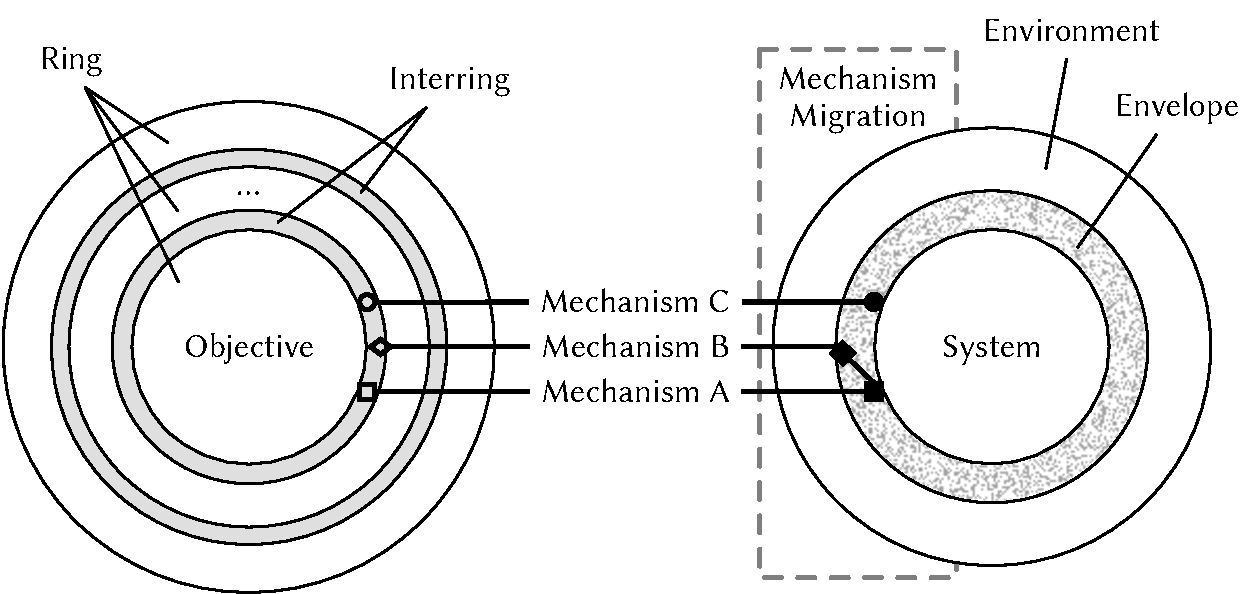
\includegraphics[width=\linewidth]{figures/MechanismMigration.pdf}
    \caption{Mechanism migration to a legacy device with transition-enabled environment}
    \label{fig:bigpicture}
\end{figure}

The concept of \emph{\mm} allows altering behavior of information and communications system (ICS) that are incapable or unwilling to modify their own operation.
This could be due to an ICS being built upon proprietary frameworks disallowing modification of the device, manufacturers dropping support or by the unwillingness to make the effort to adapt or update the components of the ICS.
In such cases developers or network operators are unable to modify the ICS itself.
However, the proposed approach of \mm enables the modification of an ICS's environment to enforce the desired adaption in its behavior.
This change can be thought of as an ''outer'' level of the communication infrastructure enveloping an ''inner'' level.

For example, when faced with a closed application executed on a smartphone, operating system (OS) might be modified to force the applications behavior to change by modifying the OS network stack to transparently wrap connection in a VPN.
If a whole device is unmodifiable, but the network is under control of the network operator the network can be utilized to force the device to behave in a desired way, e.g. by placing gateway-servers inside the network who can transparently alter traffic flows.
If even the network is outside control modifying or replacing the communication partner/backend with which the device is communicating is possible.


\subsection{Rings}
As the above examples suggest, modern information and communications technology consists of a multitude of components like access devices (smartphones, computers, etc.) and network infrastructure (routers, back-bone network), software (e.g., OSs, middle-ware, applications), networks, network topologies, network protocols on various layers, compute facilities (cloud, edge, etc.) and so on.
We subdivide these components into a ring structure, as shown in \Cref{fig:bigpicture}, where each \emph{ring} represents a component required for the given domain.
The most specific component, whose functionality is to be improved by the proposed \mm, forms the center of the structure, called \emph{objective}, while other components are added as rings.
As an example, an ICS providing a VoIP service to users, the telephony application installed on the end-users device would form the objective, as it should be modified in some way.
This application requires the OS and its networking APIs, which forms the ring around the application, whereas the next outer ring forms the local area network.
This categorization allows arbitrary deep rings that seem appropriate for the given domain.
In the above example, the outer most ring would be the backend executed on a server in the cloud.
For enabling \mm, it is important to be able to modify or alter rings around the objective, although it is not required to have control of all rings but only the ring required to achieve the desired result.


\subsection{Interrings}
Between adjacent rings, components require interaction.
Such an interface can be anything from set of rules governing the actual communication, such as protocols defined on the different layers of the network-stack-model, to implicit assumptions over the inner workings of peers in a network.
In the above example, the telephony application uses the OS's networking API to send and receive data.
Thereon, the OS uses for example Wi-Fi or cellular connectivity to access the local area network, and so on.
These interaction layers are called \emph{interrings} and are represented as gray layers between the rings in \Cref{fig:bigpicture}.
Beyond the network stack on a local device itself, interrings include any functionality that allows interaction between two rings like system calls in an application-OS relation or communications between multiple nodes in a network.


\subsection{Mechanism}
A \emph{mechanism} is a functional part of an interring that realizes functional units to achieve the desired functionality of the objective.
Examples of such mechanisms are manifold and span all protocol- and system-layers, as the following selection of possible mechanisms shows:

\begin{itemize}
 \item Complete protocols: TCP, UDP, RTP, overlays, etc.
 \item Specific parts of protocols: congestion control, fragmentation, load balancing, replication, etc.
 \item Network concepts: infrastructure-based, ad-hoc, partially meshed, delay tolerant (DTN), etc.
 \item Network technologies: Ethernet, LTE, IEEE 802.11, Bluetooth, etc.
 \item Security mechanisms: encryption, integrity protection, authentication, etc.
 \item System components: positioning (via WLAN, GSM or GPS), sensors, etc.
\end{itemize}

 

\subsection{Envelope, System and Environment}
In order to realize the proposed approach, it is necessary to migrate novel functionality to existing ICS.
An \emph{\env} is a component containing such a new or alternative mechanism that is migrated to the interring between the last ring that is under control and the first ring that is not under control.
For example, if the telephony application that should support vertical handovers is not modifiable but the OS, the \env containing a mechanism enabling vertical handovers could be placed in the interring between application and the OS.
It might also be desirable to migrate an \env into an outer interring, although a ring closer to the objective might be still under control.
All rings, including the objective, that are located within the \env are summarized as the \emph{system} and all rings outside the \env are called \emph{environment}.

 